% !TEX root = ../discretemath.tex

\section{Деревья и леса. Остовные деревья. Многочлен Татта}

\begin{Statement}{Эквивалентные определения деревьев.}{}
	Пусть $G=(V,E)$ — конечный неориентированный граф, $|V|=n$.
	Следующие утверждения эквивалентны:
	\begin{enumerate}
		\item[(i)] $G$ — дерево.
		\item[(ii)] Между любыми двумя вершинами $u,v\in V$ существует ровно один (простой) путь.
		\item[(iii)] $G$ связен и $|E|=n-1$.
		\item[(iv)] $G$ связен и при удалении любого ребра связность теряется.
	\end{enumerate}
\end{Statement}

\begin{proof}
	Напомним: \emph{дерево} — это связный граф без циклов.
	
	\smallskip
	\noindent\textbf{(i)$\Rightarrow$(ii).}
	Связность даёт существование пути между $u$ и $v$.
	Если бы существовали два различных пути, то их объединение содержало бы цикл, что противоречит ацикличности дерева.
	Значит, путь единственный.
	
	\smallskip
	\noindent\textbf{(ii)$\Rightarrow$(iv).}
	Возьмём ребро $e=xy$. В графе $G\setminus e$ не может остаться путь между $x$ и $y$,
	иначе в исходном $G$ были бы два разных пути между $x$ и $y$,
	что противоречит (ii). Значит, удаление любого ребра нарушает связность.
	
	\smallskip
	\noindent\textbf{(iv)$\Rightarrow$(i).}
	Покажем, что циклов нет. Если в $G$ есть цикл, то любое ребро цикла можно удалить,
	и вершины цикла всё равно останутся соединены обходом по оставшейся части цикла,
	то есть связность не потеряется — противоречие (iv). Значит, $G$ связен и ацикличен, то есть дерево.
	
	\smallskip
	\noindent\textbf{(i)$\Rightarrow$(iii).}
	Докажем по индукции по $n$. При $n=1$ имеем $|E|=0=n-1$.
	Пусть для всех деревьев на $n-1$ вершинах верно $|E|=(n-1)-1$.
	В любом дереве есть лист. Удалим лист и инцидентное ему ребро:
	получим дерево на $n-1$ вершинах, у которого рёбер $|E|-1$.
	По предположению индукции $|E|-1=(n-1)-1$, значит $|E|=n-1$.
	
	\smallskip
	\noindent\textbf{(iii)$\Rightarrow$(i).}
	Если в связном графе $|E|=n-1$, то циклов быть не может:
	иначе удалим ребро из цикла — граф останется связным, но рёбер станет $n-2$.
	Однако связный граф на $n$ вершинах не может иметь меньше $n-1$ рёбер (например, любое остовное дерево имеет $n-1$ ребро).
	Противоречие. Следовательно, $G$ связен и ацикличен, то есть дерево.

\end{proof}

\begin{Definition}{Лист}{}
	Пусть $G=(V,E)$ — дерево. Вершина $u\in V$ называется \emph{листом},
	если $\deg(u)=1$.
\end{Definition}

\begin{Statement}{}{}
	Если $G$ — дерево на $n\ge 2$ вершинах, то в $G$ есть хотя бы два листа.
\end{Statement}


	\noindent
	\begin{minipage}[t]{0.45\textwidth}
		\vspace{0pt}
		\centering
		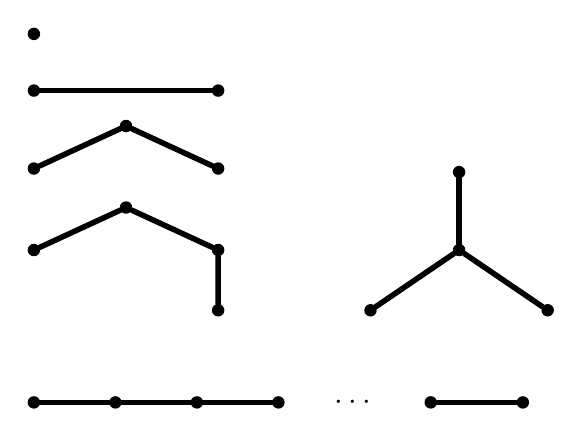
\begin{tikzpicture}[
			scale=0.45, transform shape,
			x=1cm, y=1cm,
			line cap=round, line join=round,
			dot/.style={circle, fill=black, inner sep=0pt, minimum size=10pt},
			edge/.style={draw=black, line width=2pt}
			]
			
			\node[dot] at (0,7.2) {};
			
			\node[dot] (a) at (0,5.6) {};
			\node[dot] (b) at (5.2,5.6) {};
			\draw[edge] (a)--(b);
			
			\node[dot] (c1) at (0,3.4) {};
			\node[dot] (c2) at (2.6,4.6) {};
			\node[dot] (c3) at (5.2,3.4) {};
			\draw[edge] (c1)--(c2)--(c3);
			
			\node[dot] (d1) at (0,1.1) {};
			\node[dot] (d2) at (2.6,2.3) {};
			\node[dot] (d3) at (5.2,1.1) {};
			\node[dot] (d4) at (5.2,-0.6) {};
			\draw[edge] (d1)--(d2)--(d3)--(d4);
			
			\node[dot] (e0) at (12,1.1) {};
			\node[dot] (e1) at (12,3.3) {};
			\node[dot] (e2) at (9.5,-0.6) {};
			\node[dot] (e3) at (14.5,-0.6) {};
			\draw[edge] (e0)--(e1);
			\draw[edge] (e0)--(e2);
			\draw[edge] (e0)--(e3);
			
			\node[dot] (p0) at (0,-3.2) {};
			\node[dot] (p1) at (2.3,-3.2) {};
			\node[dot] (p2) at (4.6,-3.2) {};
			\node[dot] (p3) at (6.9,-3.2) {};
			\draw[edge] (p0)--(p1)--(p2)--(p3);
			
			\node at (9.0,-3.2) {\Huge$\cdots$};
			
			\node[dot] (q0) at (11.2,-3.2) {};
			\node[dot] (q1) at (13.8,-3.2) {};
			\draw[edge] (q0)--(q1);
		\end{tikzpicture}
	\end{minipage}
	\hfill
	\begin{minipage}[t]{0.52\textwidth}
		\vspace{0pt}
		\textbf{Доказательство.}
		
		Обозначим через $L$ множество листьев и положим $\ell:=|L|$.
		Так как $G$ — дерево на $n$ вершинах, то $|E|=n-1$, поэтому по лемме о рукопожатиях
		\[
		\sum_{v\in V}\deg(v)=2|E|=2n-2.
		\]
	\end{minipage}
	
	\medskip
	\noindent
	С другой стороны, для листьев $\deg(v)=1$, а для всех остальных вершин (не листьев)
	в дереве обязательно $\deg(v)\ge 2$. Значит,
	\[
	\sum_{v\in V}\deg(v)\;\ge\;\underbrace{\ell\cdot 1}_{\text{листья}}
	\;+\;\underbrace{(n-\ell)\cdot 2}_{\text{прочие}}
	\;=\;\ell+2(n-\ell)=2n-\ell.
	\]
	Сравнивая полученные выражения, имеем:
	\[
	2n-2 = \sum_{v\in V}\deg(v) \ge 2n-\ell \quad\Longrightarrow\quad \ell\ge 2.
	\]
	То есть в дереве $G$ всегда найдется хотя бы два листа.

\begin{Theorem}{Существование остовного дерева}{}
	Пусть $G=(V,E)$ — связный граф. Тогда из $G$ можно выкинуть некоторые рёбра
	(не удаляя вершин) так, что оставшийся подграф будет деревом.
\end{Theorem}

\begin{proof}
	Пока в графе есть цикл, выберем в этом цикле ребро $e$ и удалим его.
	Удаление ребра из цикла не нарушает связность (между концами $e$ остаётся обход по остальной части цикла),
	значит граф всё ещё связен. Так как рёбер конечное число, процесс остановится.
	В конце получим связный граф без циклов, то есть дерево.
\end{proof}

\begin{Definition}{Остовное дерево}{}
	Подграф $T\subseteq G$ называется \emph{остовным деревом} графа $G$,
	если $T$ — дерево и $V(T)=V(G)$ (то есть содержит все вершины $G$).
\end{Definition}

\begin{Definition}{Лес}{}
	Граф $F=(V,E)$ называется \emph{лесом}, если он не содержит циклов.
\end{Definition}

\begin{Statement}{Эквивалентные определения леса}{}
	Пусть $F=(V,E)$ — конечный неориентированный граф, а $c(F)$ — число его компонент связности.
	Следующие утверждения эквивалентны:
	\begin{enumerate}
		\item[(i)] $F$ не содержит циклов (то есть $F$ — лес);
		\item[(ii)] $|E| = |V| - c(F)$;
		\item[(iii)] при удалении любого ребра число компонент связности увеличивается;
		\item[(iv)] каждая компонента связности графа $F$ является деревом.
	\end{enumerate}
\end{Statement}

\begin{Statement}{Удаление–стягивание}{}
	Пусть $G$ — граф, $e\in E(G)$ — ребро, которое \emph{не является петлёй}.
	Тогда для хроматического многочлена выполняется
	\[
	\chi_G(x)=\chi_{G-e}(x)-\chi_{G \cdot e}(x),
	\]
	где $G-e$ — граф с удалённым ребром $e$, а $G \cdot e$ — граф, полученный стягиванием ребра $e$.
\end{Statement}

\begin{Definition}{Мост}{}
	Ребро $e\in E(G)$ называется \emph{мостом}, если
	\[
	c(G-e) > c(G),
	\]
	то есть после удаления $e$ число компонент связности увеличивается.
\end{Definition}

	Пусть $G=(V,E)$ — граф, $e\in E$.
	Обозначим через $G-e$ граф с удалённым ребром $e$,
	а через $G \cdot e$ граф, полученный \emph{стягиванием} ребра $e$.


\begin{Proposition}{Удаление–стягивание для деревьев и лесов}{}
	Пусть $e$ \textbf{не является петлёй}. Тогда:
	\[
	\#\{\text{остовных деревьев в }G\}
	=
	\#\{\text{деревьев в }G-e\}
	+
	\#\{\text{деревьев в }G\cdot e\},
	\]
	\[
	\#\{\text{остовных лесов в }G\}
	=
	\#\{\text{остовных лесов в }G-e\}
	+
	\#\{\text{остовных лесов в }G \cdot e\}.
	\]
\end{Proposition}

\begin{Definition}{Многочлен Татта}{}
	Многочлен Татта $T_G(x,y)$ графа $G$ определяется рекурсией по ребру $e\in E(G)$:
	\begin{enumerate}
		\item[(i)] если $e$ не петля и не мост, то
		\[
		T_G(x,y)=T_{G-e}(x,y)+T_{G \cdot e}(x,y);
		\]
		\item[(ii)] если $e$ — петля, то
		\[
		T_G(x,y)=y\,T_{G-e}(x,y);
		\]
		\item[(iii)] если $e$ — мост, то
		\[
		T_G(x,y)=x\,T_{G-e}(x,y);
		\]
		\item[(iv)] если $G$ пустой (без рёбер), то
		\[
		T_G(x,y)=1.
		\]
	\end{enumerate}
\end{Definition}

\begin{Proposition}{}{}
	Определение корректно: $T_G(x,y)$ не зависит от выбора ребра $e$ и порядка применения рекурсии.
\end{Proposition}

\begin{proof}
	Зафиксируем некоторый порядок рёбер $E(G)=\{e_1,\dots,e_m\}$ и будем раскрывать рекурсию,
	последовательно «обрабатывая» рёбра в этом порядке.
	Нужно доказать, что при любом другом порядке получится тот же многочлен.
	
	Достаточно проверить, что результат не меняется при \emph{перестановке двух соседних рёбер}
	(так как любая перестановка раскладывается в произведение соседних транспозиций).
	То есть достаточно сравнить два порядка:
	\[
	e_1,\dots,e_i,e_{i+1},\dots,e_m
	\quad\text{и}\quad
	e_1,\dots,e_{i+1},e_i,\dots,e_m.
	\]
	
	Обозначим через $G'$ граф, который получается после того, как мы уже обработали рёбра
	$e_1,\dots,e_{i-1}$.
	
	По предположению индукции по числу оставшихся рёбер
	достаточно проверить, что \emph{в одном и том же} графе $G'$ обработка $e_i$ и $e_{i+1}$
	коммутирует.
	
	\medskip
	\noindent\textbf{0) Если $e_i$ и $e_{i+1}$ кратные, то очевидно:}
	локально получаются одни и те же графы после удаления/стягивания,
	и результат совпадает.
	
	\smallskip
	\noindent\textbf{1) Если $e_i$ или $e_{i+1}$ — петля, то тоже очевидно:}
	для петли действует правило $T_{G'}=y\,T_{G'-e}$, множитель $y$ можно вынести,
	и он не зависит от того, какое из двух рёбер обрабатывали первым.
	
	\medskip
	Далее считаем, что $e_i$ и $e_{i+1}$ \textbf{не кратные и не петли} в $G'$.
	
	\medskip
	\noindent\textbf{2) Если $e_i$ или $e_{i+1}$ — мост, то всё просто.}
	Например, если $e_{i+1}$ — мост в $G'$, то
	\[
	T_{G'}=x\,T_{G'-e_{i+1}},
	\]
	и дальнейшая обработка $e_i$ происходит уже внутри $G'-e_{i+1}$, при этом множитель $x$
	не зависит от порядка обработки этих двух рёбер. Аналогично, если мостом является $e_i$.
	
	\medskip
	\noindent\textbf{3) Пусть $e_i$ и $e_{i+1}$ не мосты в $G'$.}
	Рассмотрим два подслучая.
	
	\smallskip
	\noindent\textbf{3.1) $c(G'-e_i-e_{i+1})=c(G')$.}
	Тогда оба ребра остаются «обычными» (не мостами и не петлями) при переходах,
	и можно просто раскрыть рекурсию в обоих порядках.
	Сначала обработаем $e_{i+1}$:
	\begin{align*}
		T_{G'}
		&=T_{G'-e_{i+1}}+T_{G'\cdot e_{i+1}}\\
		&=\Bigl(T_{G'-e_i-e_{i+1}}+T_{(G'-e_{i+1})\cdot e_i}\Bigr)
		+\Bigl(T_{(G'\cdot e_{i+1})-e_i}+T_{(G'\cdot e_{i+1})\cdot e_i}\Bigr).
	\end{align*}
	Теперь используем коммутативность удаления/стягивания для различных рёбер:
	\[
	(G'-e_{i+1})\cdot e_i \cong (G'\cdot e_i)-e_{i+1},\qquad
	(G'\cdot e_{i+1})-e_i \cong (G'-e_i)\cdot e_{i+1},\qquad
	(G'\cdot e_{i+1})\cdot e_i \cong (G'\cdot e_i)\cdot e_{i+1}.
	\]
	Тогда получаем симметричную сумму из четырёх одинаковых графов:
	\[
	T_{G'}
	=
	T_{G'-e_i-e_{i+1}}
	+T_{(G'-e_i)\cdot e_{i+1}}
	+T_{(G'\cdot e_i)-e_{i+1}}
	+T_{(G'\cdot e_i)\cdot e_{i+1}},
	\]
	что ровно совпадает с раскрытием рекурсии в порядке $e_i$ затем $e_{i+1}$.
	Значит, в этом подслучае порядок не важен.
	
	\smallskip
	\noindent\textbf{3.2) $c(G'-e_i-e_{i+1})=c(G')+1$.}
	То есть по отдельности $e_i$ и $e_{i+1}$ не мосты, но удаление \emph{обоих} рёбер увеличивает число компонент.
	Тогда, например, в графе $G'-e_{i+1}$ ребро $e_i$ становится мостом (и симметрично наоборот), поэтому
	\begin{align*}
		T_{G'}
		&=T_{G'-e_{i+1}}+T_{G' \cdot e_{i+1}}
		= x\,T_{G'-e_i-e_{i+1}} \;+\; T_{G'\cdot e_{i+1}},\\
		T_{G'\cdot e_{i+1}}
		&= T_{(G'\cdot e_{i+1})-e_i}+T_{(G' \cdot e_{i+1})\cdot e_i}.
	\end{align*}
	Итак,
	\[
	T_{G'}
	=
	x\,T_{G'-e_i-e_{i+1}}
	+T_{(G'\cdot e_{i+1})-e_i}
	+T_{(G'\cdot e_{i+1})\cdot e_i}.
	\]
	Аналогично при раскрытии сначала по $e_i$, потом по $e_{i+1}$:
	\[
	T_{G'}
	=
	x\,T_{G'-e_i-e_{i+1}}
	+T_{(G'\cdot e_i)-e_{i+1}}
	+T_{(G'\cdot e_i)\cdot e_{i+1}}.
	\]
	
	\vspace{-0.6em}
	\begin{center}
		\setlength{\abovecaptionskip}{0pt}
		\setlength{\belowcaptionskip}{0pt}
		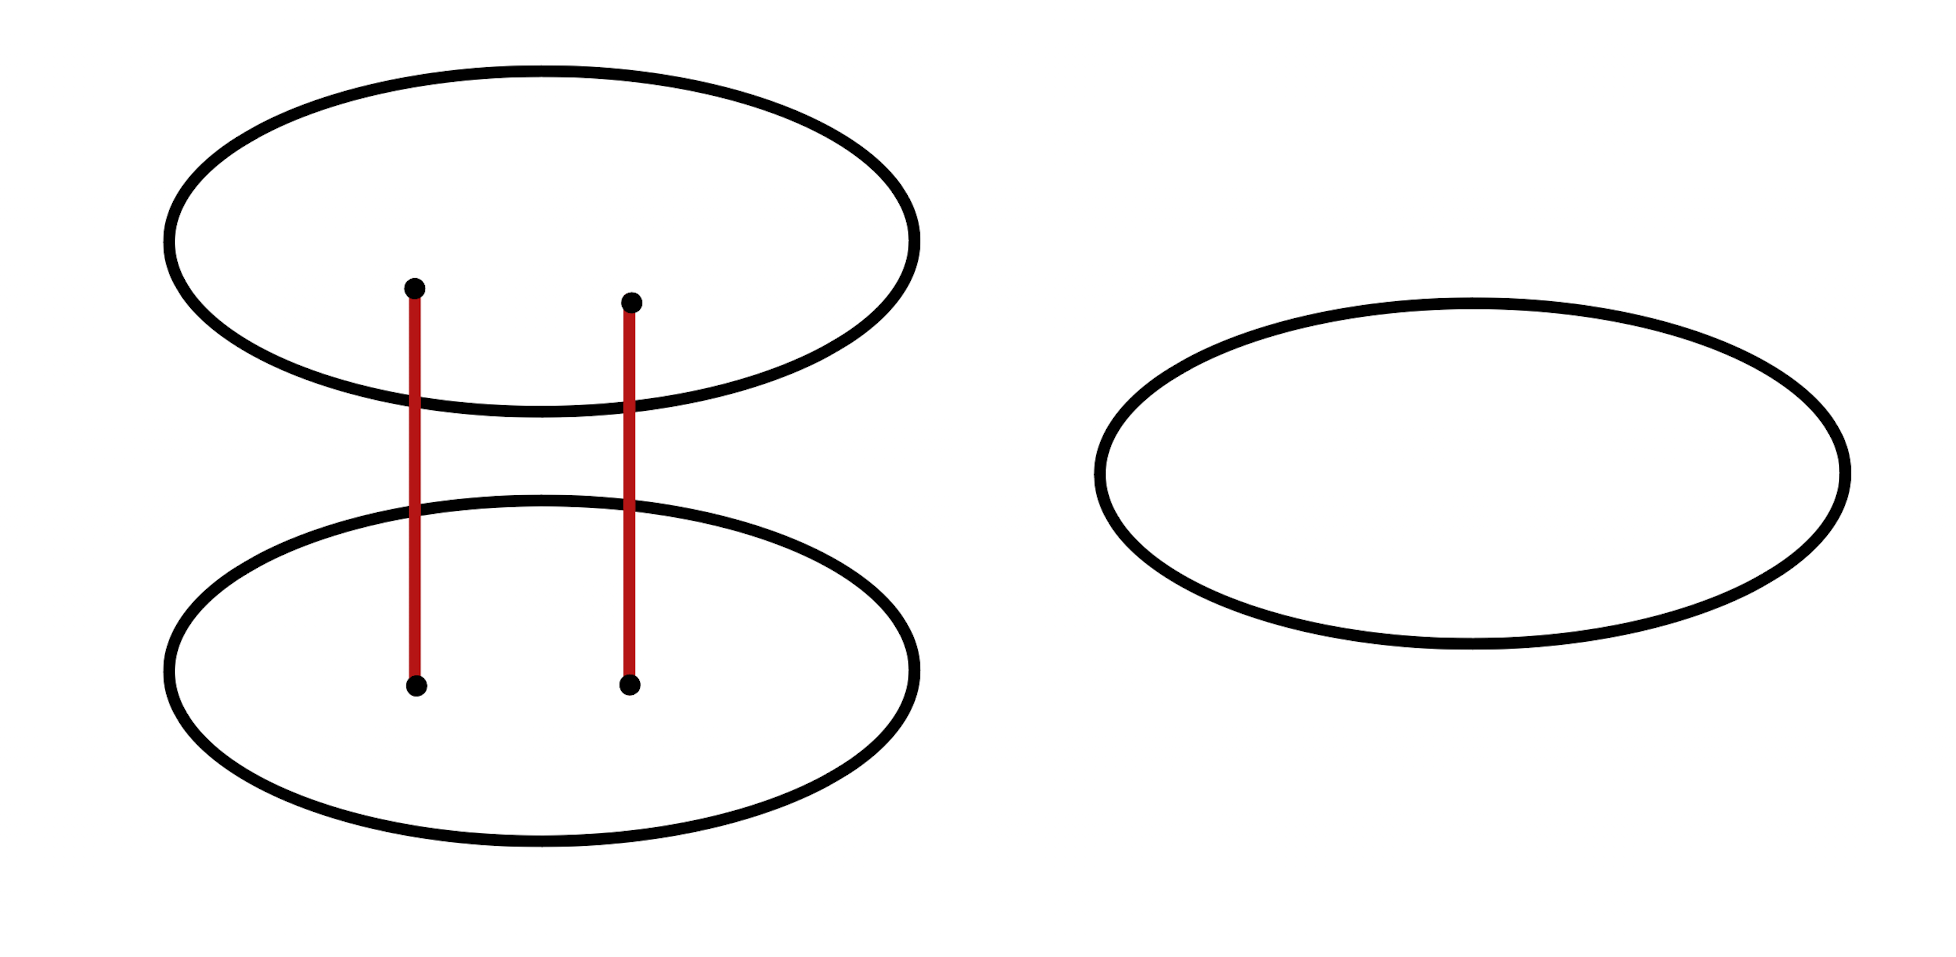
\includegraphics[width=0.38\linewidth]{img/pol_tutte_1.png}\par\vspace{0.35em}
		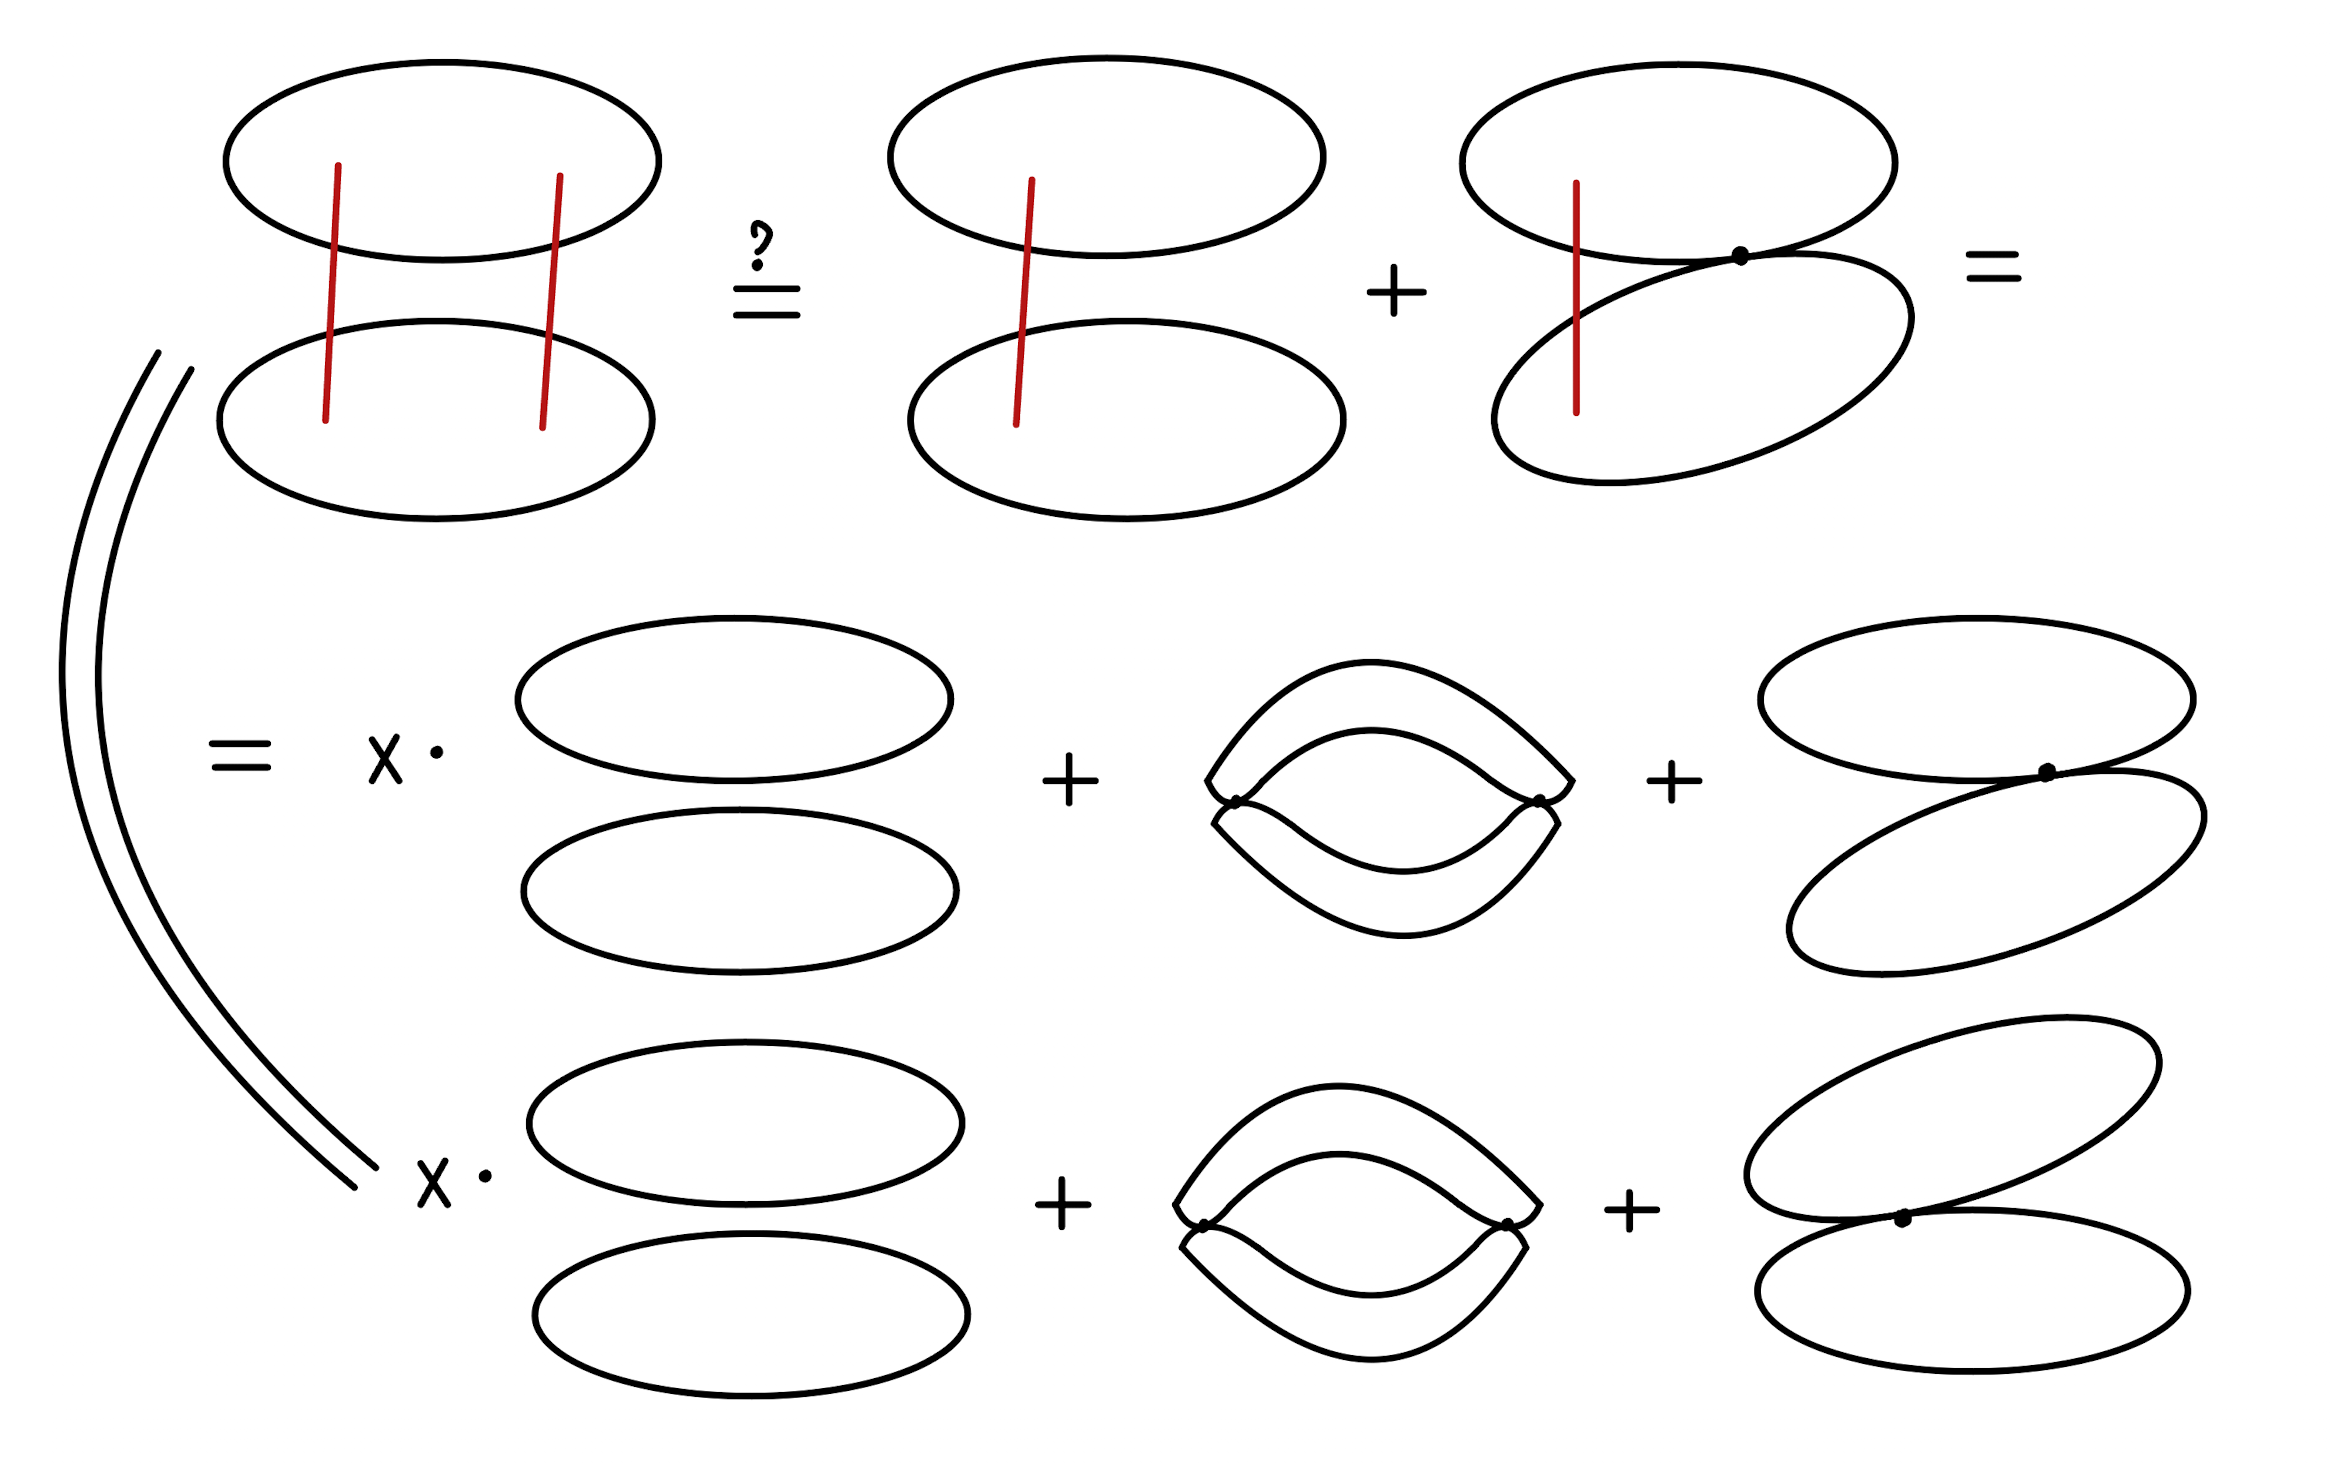
\includegraphics[width=0.60\linewidth]{img/pol_tutte_2.png}
	\end{center}
	\vspace{-0.6em}
	
	Оставшиеся два слагаемых совпадают, так как для различных рёбер операции удаления и стягивания коммутируют:
	\[
	(G'\cdot e_{i+1})-e_i \cong (G'\cdot e_i)-e_{i+1},
	\qquad
	(G'\cdot e_{i+1})\cdot e_i \cong (G'\cdot e_i)\cdot e_{i+1}.
	\]
	Следовательно, раскрытие рекурсии в двух порядках даёт один и тот же результат.

\end{proof}

\begin{Theorem}{Формула по подмножествам}{}
	Для любого графа $G=(V,E)$ многочлен Татта равен
	\[
	T_G(x,y)=\sum_{A\subseteq E}
	(x-1)^{\,c(A)-c(E)}\,(y-1)^{\,c(A)+|A|-|V|}.
	\]
\end{Theorem}

\begin{Remark}{}{}
	Пусть $G=(V,E)$ — конечный граф. Для $A\subseteq E$ обозначим через
	$c(A)$ число компонент связности в остовном подграфе $(V,A)$.
	В частности, $c(E)=c(G)$.
\end{Remark}

\begin{proof}
	Обозначим правую часть через
	\[
	F_G(x,y):=\sum_{A\subseteq E}
	(x-1)^{\,c(A)-c(E)}(y-1)^{\,c(A)+|A|-|V|}.
	\]
	Покажем, что $F_G$ удовлетворяет той же рекурсии удаления--стягивания и той же базе,
	что и $T_G$. Тогда $F_G\equiv T_G$.
	
	\smallskip
	\noindent\textbf{База:} если $E=\varnothing$, то единственное подмножество $A=\varnothing$,
	и $c(\varnothing)=|V|=c(E)$, поэтому $F_G=1$, как и по определению $T_G$.
	
	\smallskip
	\noindent\textbf{Шаг:} возьмём ребро $e\in E$ и разложим сумму по случаям $e\notin A$ и $e\in A$:
	\begin{align*}
		F_G
		&=\sum_{A\subseteq E\setminus\{e\}}
		(x-1)^{c(A)-c(E)}(y-1)^{c(A)+|A|-|V|} \\
		&\quad+\sum_{A\subseteq E\setminus\{e\}}
		(x-1)^{c(A\cup\{e\})-c(E)}(y-1)^{c(A\cup\{e\})+|A|+1-|V|}.
	\end{align*}
	
	\medskip
	\noindent\textbf{1) $e$ — мост.}
	Тогда $c(E\setminus\{e\})=c(E)+1$.
	Кроме того, для любого $A\subseteq E\setminus\{e\}$ добавление моста уменьшает число компонент на $1$:
	$c(A\cup\{e\})=c(A)-1$.
	Поэтому второй сумме соответствует
	\[
	(x-1)^{c(A\cup\{e\})-c(E)}=(x-1)^{c(A)-1-c(E)}=(x-1)^{c(A)-c(E\setminus\{e\})},
	\]
	а показатель у $(y-1)$ упрощается:
	\[
	c(A\cup\{e\})+|A|+1-|V|=(c(A)-1)+|A|+1-|V|=c(A)+|A|-|V|.
	\]
	Значит, вторая сумма равна $F_{G-e}$.
	
	Первая сумма отличается от $F_{G-e}$ ровно дополнительным множителем $(x-1)$,
	потому что в $F_{G-e}$ стоит степень $(x-1)^{c(A)-c(E\setminus\{e\})}$, а здесь
	$(x-1)^{c(A)-c(E)}=(x-1)\cdot (x-1)^{c(A)-c(E\setminus\{e\})}$.
	Итого
	\[
	F_G=(x-1)F_{G-e}+F_{G-e}=x\,F_{G-e},
	\]
	что совпадает с правилом Татта для моста.
	
	\medskip
	\noindent\textbf{2) $e$ — петля.}
	Тогда $c(E\setminus\{e\})=c(E)$ и для любого $A\subseteq E\setminus\{e\}$ имеем
	$c(A\cup\{e\})=c(A)$.
	Поэтому во второй сумме показатель $(y-1)$ увеличивается на $1$, а всё остальное совпадает с первой:
	\[
	\text{(2-я сумма)}=(y-1)\,\text{(1-я сумма)}.
	\]
	Следовательно,
	\[
	F_G=F_{G-e}+(y-1)F_{G-e}=y\,F_{G-e},
	\]
	что совпадает с правилом Татта для петли.
	
	\medskip
	\noindent\textbf{3) $e$ не петля и не мост.}
	Тогда $c(E\setminus\{e\})=c(E)$, и первая сумма в точности равна $F_{G-e}$.
	
	Во второй сумме используем стандартную биекцию:
	подмножеству $A\subseteq E\setminus\{e\}$ соответствует подмножество рёбер $A^\ast\subseteq E(G/e)$, причём
	\[
	c_{G/e}(A^\ast)=c_G(A\cup\{e\}),\qquad |A^\ast|=|A|,\qquad |V(G/e)|=|V|-1,
	\]
	а также $c_{G/e}(E(G/e))=c_G(E)=c(E)$.
	Тогда вторая сумма переписывается как
	\[
	\sum_{A^\ast\subseteq E(G/e)}
	(x-1)^{c_{G/e}(A^\ast)-c_{G/e}(E(G/e))}
	(y-1)^{c_{G/e}(A^\ast)+|A^\ast|-(|V|-1)}
	=F_{G/e}.
	\]
	Значит,
	\[
	F_G=F_{G-e}+F_{G/e},
	\]
	что совпадает с правилом Татта для ребра, которое не является ни петлёй, ни мостом.
	
	\medskip
	Итак, $F_G$ удовлетворяет тем же рекурсивным соотношениям и базе, что и $T_G$,
	следовательно $F_G\equiv T_G$.
\end{proof}

\begin{Remark}{}{}
	В многочлене Татта $T_G(x,y)$ все коэффициенты — неотрицательные целые числа.
\end{Remark}

\begin{Statement}{Специализации $T_G$}{}
	Пусть $G=(V,E)$ — конечный граф.
	\begin{enumerate}
		\item $T_G(2,2)=2^{|E|}$.
		\item $T_G(2,1)$ равно числу остовных лесов графа $G$
		(то есть числу подмножеств рёбер $A\subseteq E$, для которых $(V,A)$ не содержит циклов).
		\item Если $G$ связен, то $T_G(1,1)$ равно числу остовных деревьев графа $G$.
	\end{enumerate}
\end{Statement}

\begin{Theorem}{Связь с хроматическим многочленом}{}
	Пусть $X_G(n)$ — хроматический многочлен графа $G$, а $c(G)$ — число компонент связности.
	Тогда
	\[
	X_G(n)=(-1)^{|V|-c(G)}\,n^{c(G)}\,T_G(1-n,0).
	\]
\end{Theorem}

\begin{proof}
	Обозначим
	\[
	F_G(n):=(-1)^{|V|-c(G)}\,n^{c(G)}\,T_G(1-n,0).
	\]
	Покажем, что $F_G(n)$ удовлетворяет тем же рекурсиям и базе, что и $X_G(n)$.
	
	\smallskip
	\noindent\textbf{База:} если $E=\varnothing$, то $T_G(x,y)=1$, и
	\[
	F_G(n)=(-1)^{|V|-|V|}\,n^{|V|}\cdot 1=n^{|V|}=X_G(n).
	\]
	
	\smallskip
	\noindent\textbf{Случай 1: $e$ — петля.}
	Тогда $X_G(n)=0$. Для Татта при петле $T_G(x,y)=y\,T_{G-e}(x,y)$, значит при $y=0$
	получаем $T_G(1-n,0)=0$, то есть $F_G(n)=0=X_G(n)$.
	
	\smallskip
	\noindent\textbf{Случай 2: $e$ — мост.}
	Тогда $G-e$ имеет на одну компоненту больше: $c(G-e)=c(G)+1$, и для Татта
	$T_G(x,y)=x\,T_{G-e}(x,y)$. Кроме того, для хроматического многочлена верно
	\[
	X_G(n)=\frac{n-1}{n}\,X_{G-e}(n)
	\]
	(так как в $G-e$ две компоненты раскрашиваются независимо, а концы моста должны иметь разные цвета;
	для фиксированной раскраски одной компоненты вероятность совпадения цвета конца во второй равна $1/n$).
	
	Проверим то же для $F_G$:
	\begin{align*}
		F_G(n)
		&=(-1)^{|V|-c(G)}n^{c(G)}\,(1-n)\,T_{G-e}(1-n,0)\\
		&=\frac{n-1}{n}\;(-1)^{|V|-c(G-e)}n^{c(G-e)}\,T_{G-e}(1-n,0)
		=\frac{n-1}{n}\,F_{G-e}(n).
	\end{align*}
	Значит, в мостовом случае рекурсия совпадает с рекурсией для $X_G$.
	
	\smallskip
	\noindent\textbf{Случай 3: $e$ не петля и не мост.}
	Тогда выполняются рекурсии
	\[
	X_G(n)=X_{G-e}(n)-X_{G/e}(n),
	\qquad
	T_G(x,y)=T_{G-e}(x,y)+T_{G/e}(x,y).
	\]
	При этом $c(G-e)=c(G)$ и $c(G/e)=c(G)$, а $|V(G/e)|=|V|-1$. Поэтому
	\begin{align*}
		F_G(n)
		&=(-1)^{|V|-c(G)}n^{c(G)}\bigl(T_{G-e}(1-n,0)+T_{G/e}(1-n,0)\bigr)\\
		&=F_{G-e}(n)\;-\;F_{G/e}(n),
	\end{align*}
	поскольку переход $G\mapsto G/e$ уменьшает $|V|$ на $1$ и даёт дополнительный минус.
	Значит, $F_G$ удовлетворяет той же рекурсии, что и $X_G$.
	
	\smallskip
	Итак, $F_G(n)$ и $X_G(n)$ совпадают на базе и удовлетворяют одинаковым рекурсиям,
	следовательно $F_G(n)\equiv X_G(n)$.
\end{proof}